% \iffalse
\let\negmedspace\undefined
\let\negthickspace\undefined
\documentclass[journal,12pt,twocolumn]{IEEEtran}
\usepackage{cite}
\usepackage{amsmath,amssymb,amsfonts,amsthm}
\usepackage{algorithmic}
\usepackage{graphicx}
\usepackage{textcomp}
\usepackage{xcolor}
\usepackage{txfonts}
\usepackage{listings}
\usepackage{enumitem}
\usepackage{mathtools}
\usepackage{gensymb}
\usepackage{comment}
\usepackage[breaklinks=true]{hyperref}
\usepackage{tkz-euclide} 
\usepackage{listings}
\usepackage{gvv}                                        
\def\inputGnumericTable{}                                 
\usepackage[latin1]{inputenc}                                
\usepackage{color}                                            
\usepackage{array}                                            
\usepackage{longtable}                                       
\usepackage{calc}                                             
\usepackage{multirow}                                         
\usepackage{hhline}                                           
\usepackage{ifthen}                                           
\usepackage{lscape}
\usepackage{placeins}
\usepackage{xparse}


\newtheorem{theorem}{Theorem}[section]
\newtheorem{problem}{Problem}
\newtheorem{proposition}{Proposition}[section]
\newtheorem{lemma}{Lemma}[section]
\newtheorem{corollary}[theorem]{Corollary}
\newtheorem{example}{Example}[section]
\newtheorem{definition}[problem]{Definition}
\newcommand{\BEQA}{\begin{eqnarray}}
\newcommand{\EEQA}{\end{eqnarray}}
\newcommand{\define}{\stackrel{\triangle}{=}}
\theoremstyle{remark}
\newtheorem{rem}{Remark}

\graphicspath{ {./figs/} } 

\begin{document}

\bibliographystyle{IEEEtran}
\vspace{3cm}

\Large\title{GATE ME 30}
\large\author{EE23BTECH11032 - Kaustubh Parag Khachane $^{*}$% <-this % stops a space
}
\maketitle
\newpage
\bigskip

\renewcommand{\thefigure}{\theenumi}
\renewcommand{\thetable}{\theenumi}
\large\textbf{Question GATE ME 30} :\\
The figure shows a block of mass m = 20 kg attached to a pair of identical linear springs, each having a spring constant k = 1000 N/m. The block oscillates on a frictionless horizontal surface. Assuming free vibrations, the time taken by the block to complete ten oscillations is \rule{1cm}{0.15mm} seconds . (Rounded off to two decimal places) Take $\pi$ = 3.14. \\ \hfill(GATE ME 2023)

\begin{figure}[!ht]
\centering
\begin{center}
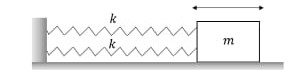
\includegraphics[width=\columnwidth]{questiondiagram}
\end{center}
%\caption{Diagram for GATE ME Question 30}
\end{figure}

\solution\\
\begin{table}[!ht] 
\centering
\setlength{\extrarowheight}{8pt}
\begin{tabular}{|l|l|l|}
    \hline
    \textbf{Parameter} & \textbf{Description} & \textbf{Value} \\
    \hline
     m & Mass of object & 10 Kg \\\hline
     $\mu$ & Frictional coefficient \brak{static} & 0.25\\\hline
     x\brak{t} & Displacement of block &  \\\hline
     $x\brak{0}$ & Initial displacement & 0 \brak{assumed} \\\hline
     g & Gravitational acceleration & 10 $m/s^2$ \\\hline
     $F_s$ & Spring force &  \\\hline
     f & frictional force &  $\mu$ N \\\hline
     N & Normal Force & mg $cos\brak{\theta}$ \\\hline
    \end{tabular}
  \vspace{4mm}
 \caption{Parameter Table}
 \label{tab:table0_xe80}
\end{table}

Derivation for natural frequency $\omega_n$:
\begin{align}
    F &= ma \\
    F &= -kx \text{ using Hooke's Law}\\
    \implies ma &= -kx\\
    \therefore m\frac{d^2x}{dt^2} &= -kx\label{eq:eq5}
\end{align}
The derivative of x has x in it's equation. So we can assume x to be of the form :
\begin{align}
    x &= Ce^{\alpha t} \label{eq:eq1}\\
    \text{Let } \frac{d^2x}{dt^2} &= -\frac{k}{m}x = -\omega^2 x \label{eq:eq2}
\end{align}
Using equations \eqref{eq:eq1} and \eqref{eq:eq2},
\begin{align}
    C\alpha^2 e^{\alpha t} &= -\omega^2 x\\
    \implies \alpha^2 &= -\omega^2\\
    \therefore \alpha &= \pm  \iota  \omega \label{eq:eq3}
\end{align}
Using \eqref{eq:eq3}, we can write x as ,
\begin{align}
    x\brak{t} = C_1e^{\iota \omega t} + C_2e^{-\iota \omega t}
\end{align}
But x always has a real value,
\begin{align}
    \therefore C_1 - C_2 &= 0  \text{ to cancel imaginary term}\\
    \implies x  &= \brak{A}\cos\brak{\omega t}\label{eq:eq4} \text{ A is a constant}
\end{align}
Observe in equation \eqref{eq:eq4}, the time period is $\frac{2\pi}{\omega}$\\
$\therefore$ $\omega$ is the natural frequency of the system.\\
From equation \eqref{eq:eq2}
\begin{align}
    \omega &= \sqrt{\frac{k}{m}}
\end{align}
using table \tabref{tab:table0} ,
\begin{align}
    k_{eq} &= 2000 \label{eq:eq6}\\
    \omega_n &= 10 rad/s\label{eq:eq7}
\end{align}
The time required to complete 10 oscillations using \eqref{eq:eq6} and \eqref{eq:eq7} is \\
\begin{align}
    10T &= 10\frac{2\pi}{\omega_n}\\
    &= 2\pi\\
    &= 6.28
\end{align}
\end{document}
